\documentclass[11pt,a4paper]{article}

% ── Packages ──────────────────────────────────────────────────────────────────
\usepackage[T1]{fontenc}
\usepackage[utf8]{inputenc}
\usepackage{helvet}
\renewcommand{\familydefault}{\sfdefault}   % Arial-like sans-serif font
\usepackage[margin=2.5cm]{geometry}
\usepackage{hyperref}
\usepackage{listingsutf8}
\usepackage{xcolor}
\usepackage{enumitem}
\usepackage{titlesec}
\usepackage{parskip}
\usepackage{booktabs}
\usepackage{graphicx}
\usepackage{amsmath}
\usepackage{fancyhdr}
\usepackage[title]{appendix}
\usepackage{tikz}
\usepackage{float}
\usepackage{caption}
\usetikzlibrary{shapes.geometric, arrows.meta, positioning, fit, backgrounds}

% ── Colors ────────────────────────────────────────────────────────────────────
\definecolor{codebg}{HTML}{F5F5F5}
\definecolor{codeframe}{HTML}{CCCCCC}
\definecolor{keyword}{HTML}{0000CC}
\definecolor{comment}{HTML}{007700}
\definecolor{string}{HTML}{CC0000}
\definecolor{uu-red}{HTML}{990000}

% ── Listings style ────────────────────────────────────────────────────────────
\lstdefinestyle{docker}{
  language=bash,
  basicstyle=\ttfamily\small,
  backgroundcolor=\color{codebg},
  frame=single,
  rulecolor=\color{codeframe},
  breaklines=true,
  breakatwhitespace=true,
  columns=fullflexible,
  keepspaces=true,
  showstringspaces=false,
  commentstyle=\color{comment},
  keywordstyle=\color{keyword}\bfseries,
  stringstyle=\color{string},
  numbers=left,
  numberstyle=\tiny\color{gray},
  numbersep=8pt,
  tabsize=2,
}

\lstdefinestyle{yaml}{
  language=bash,
  basicstyle=\ttfamily\small,
  backgroundcolor=\color{codebg},
  frame=single,
  rulecolor=\color{codeframe},
  breaklines=true,
  columns=fullflexible,
  keepspaces=true,
  showstringspaces=false,
  morecomment=[l]{\#},
  commentstyle=\color{comment},
  numbers=left,
  numberstyle=\tiny\color{gray},
  numbersep=8pt,
  tabsize=2,
}

\lstdefinestyle{shell}{
  language=bash,
  basicstyle=\ttfamily\small,
  backgroundcolor=\color{codebg},
  frame=single,
  rulecolor=\color{codeframe},
  breaklines=true,
  columns=fullflexible,
  keepspaces=true,
  showstringspaces=false,
}

\lstdefinestyle{python}{
  language=Python,
  basicstyle=\ttfamily\small,
  backgroundcolor=\color{codebg},
  frame=single,
  rulecolor=\color{codeframe},
  breaklines=true,
  breakatwhitespace=true,
  columns=fullflexible,
  keepspaces=true,
  showstringspaces=false,
  commentstyle=\color{comment},
  keywordstyle=\color{keyword}\bfseries,
  stringstyle=\color{string},
  numbers=left,
  numberstyle=\tiny\color{gray},
  numbersep=8pt,
  tabsize=4,
}

% ── Section title formatting ──────────────────────────────────────────────────
\lstset{inputencoding=utf8, extendedchars=true}
\titleformat{\section}{\large\bfseries\color{black}}{\thesection}{1em}{}
\titleformat{\subsection}{\normalsize\bfseries}{\thesubsection}{1em}{}
\titleformat{\subsubsection}{\normalsize\itshape}{\thesubsubsection}{1em}{}

% ── Header / Footer ───────────────────────────────────────────────────────────
\pagestyle{fancy}
\fancyhf{}
\lhead{\small Data Engineering II -- Assignment 4}
\rhead{\small Uppsala University}
\cfoot{\thepage}

% ── Hyperref setup ────────────────────────────────────────────────────────────
\hypersetup{
  colorlinks=true,
  linkcolor=black,
  urlcolor=blue,
}

% ── Graphics path ─────────────────────────────────────────────────────────────
\graphicspath{{figures/}}

% ─────────────────────────────────────────────────────────────────────────────
\begin{document}

% ── Title page ────────────────────────────────────────────────────────────────
\begin{titlepage}
  \centering
  \vspace*{2cm}
  {\large Uppsala University\\[0.3em]
   Department of Information Technology\\[2cm]}
  {\LARGE\bfseries Assignment 4\\[0.5em]}
  {\Large Large Scale Machine Learning\\[2cm]}
  {\large Course: Data Engineering II\\[1.5cm]}
  {\normalsize Arnab Kumar Ghosh\\[0.5cm]}
  {\normalsize \today\\[3cm]}
  \vfill
\end{titlepage}

\tableofcontents
\newpage

% =============================================================================
\section{Task 1: Distributed Machine Learning (Mandatory)}
% =============================================================================

\subsection{Infrastructure Setup}

I followed the same process I used in Assignment~3 to provision and configure the VMs.
I used the OpenStack client scripts to create the VMs on Swedish Science Cloud, and Ansible playbooks
to configure them and install the required software.
I modified both the OpenStack client scripts and the Ansible playbooks from my
Assignment~3 versions to fit this assignment -- specifically, to provision a Ray cluster
instead of a Docker-based deployment and to install Ray and scikit-learn on each node.

One VM was designated the \textbf{head node}. Ray was started on it with:

\begin{lstlisting}[style=shell]
ray start --head --port=6379 \
  --node-ip-address=<head-internal-ip> \
  --dashboard-host=0.0.0.0
\end{lstlisting}

Each additional VM joined as a \textbf{worker node} by connecting to the head:

\begin{lstlisting}[style=shell]
ray start --address='<head-internal-ip>:6379' \
  --node-ip-address=<worker-internal-ip>
\end{lstlisting}

I ran the tuning script on the head node, which distributed trials
across all connected workers via Ray's distributed scheduler and object store.
I also attached a floating IP only to the head node for SSH access. Inter-node
communication used the private network addresses.

\subsection{Task 1.1: Hyperparameter Tuning}

\subsubsection{Problem Setup with scikit-learn}

I set up the cover-type prediction problem using the \texttt{fetch\_covtype} dataset
from scikit-learn, which contains 581\,012 samples and 54 features describing cartographic
variables of forest patches in Colorado, with the goal of classifying seven forest cover types.

For the experiment, I downloaded the dataset locally to my client machine and then uploaded it to the Ray head VM through the client VM. Due to memory limits on the VM, I used only the first 20\,000 samples for each experiment. When I tried to run experiments with the full dataset, the process ran out of memory and was killed.

I instantiated a \texttt{RandomForestClassifier} with its default parameters. The full
parameter dictionary (obtained via \texttt{get\_params()}) is shown in the screenshot below.

\begin{figure}[H]
  \centering
  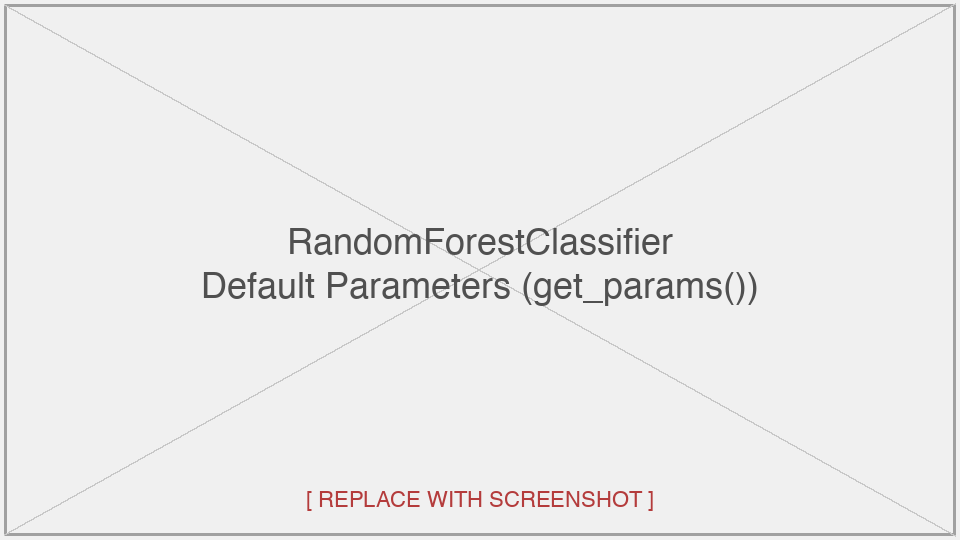
\includegraphics[width=0.95\textwidth]{screenshot-rf-params}
  \caption{Default parameters of \texttt{RandomForestClassifier} as returned by
           \texttt{get\_params()}.}
  \label{fig:rf-params}
\end{figure}

The default parameters for the \texttt{RandomForestClassifier} are:

\begin{lstlisting}[language=python, style=python]
{'bootstrap': True, 'ccp_alpha': 0.0, 'class_weight': None, 'criterion': 'gini', 
'max_depth': None, 'max_features': 'sqrt', 'max_leaf_nodes': None, 
'max_samples': None, 'min_impurity_decrease': 0.0, 'min_samples_leaf': 1, 
'min_samples_split': 2, 'min_weight_fraction_leaf': 0.0, 'monotonic_cst': None, 
'n_estimators': 100, 'n_jobs': None, 'oob_score': False, 'random_state': 42, 
'verbose': 0, 'warm_start': False}
\end{lstlisting}

I evaluated the model using 3-fold cross-validation on the 20,000-sample subset, obtaining a mean
accuracy of \textbf{0.7025} in a runtime of approximately 7.60 seconds.
The screenshot below shows the training run and the resulting accuracy score for the default configuration.

\begin{figure}[H]
  \centering
  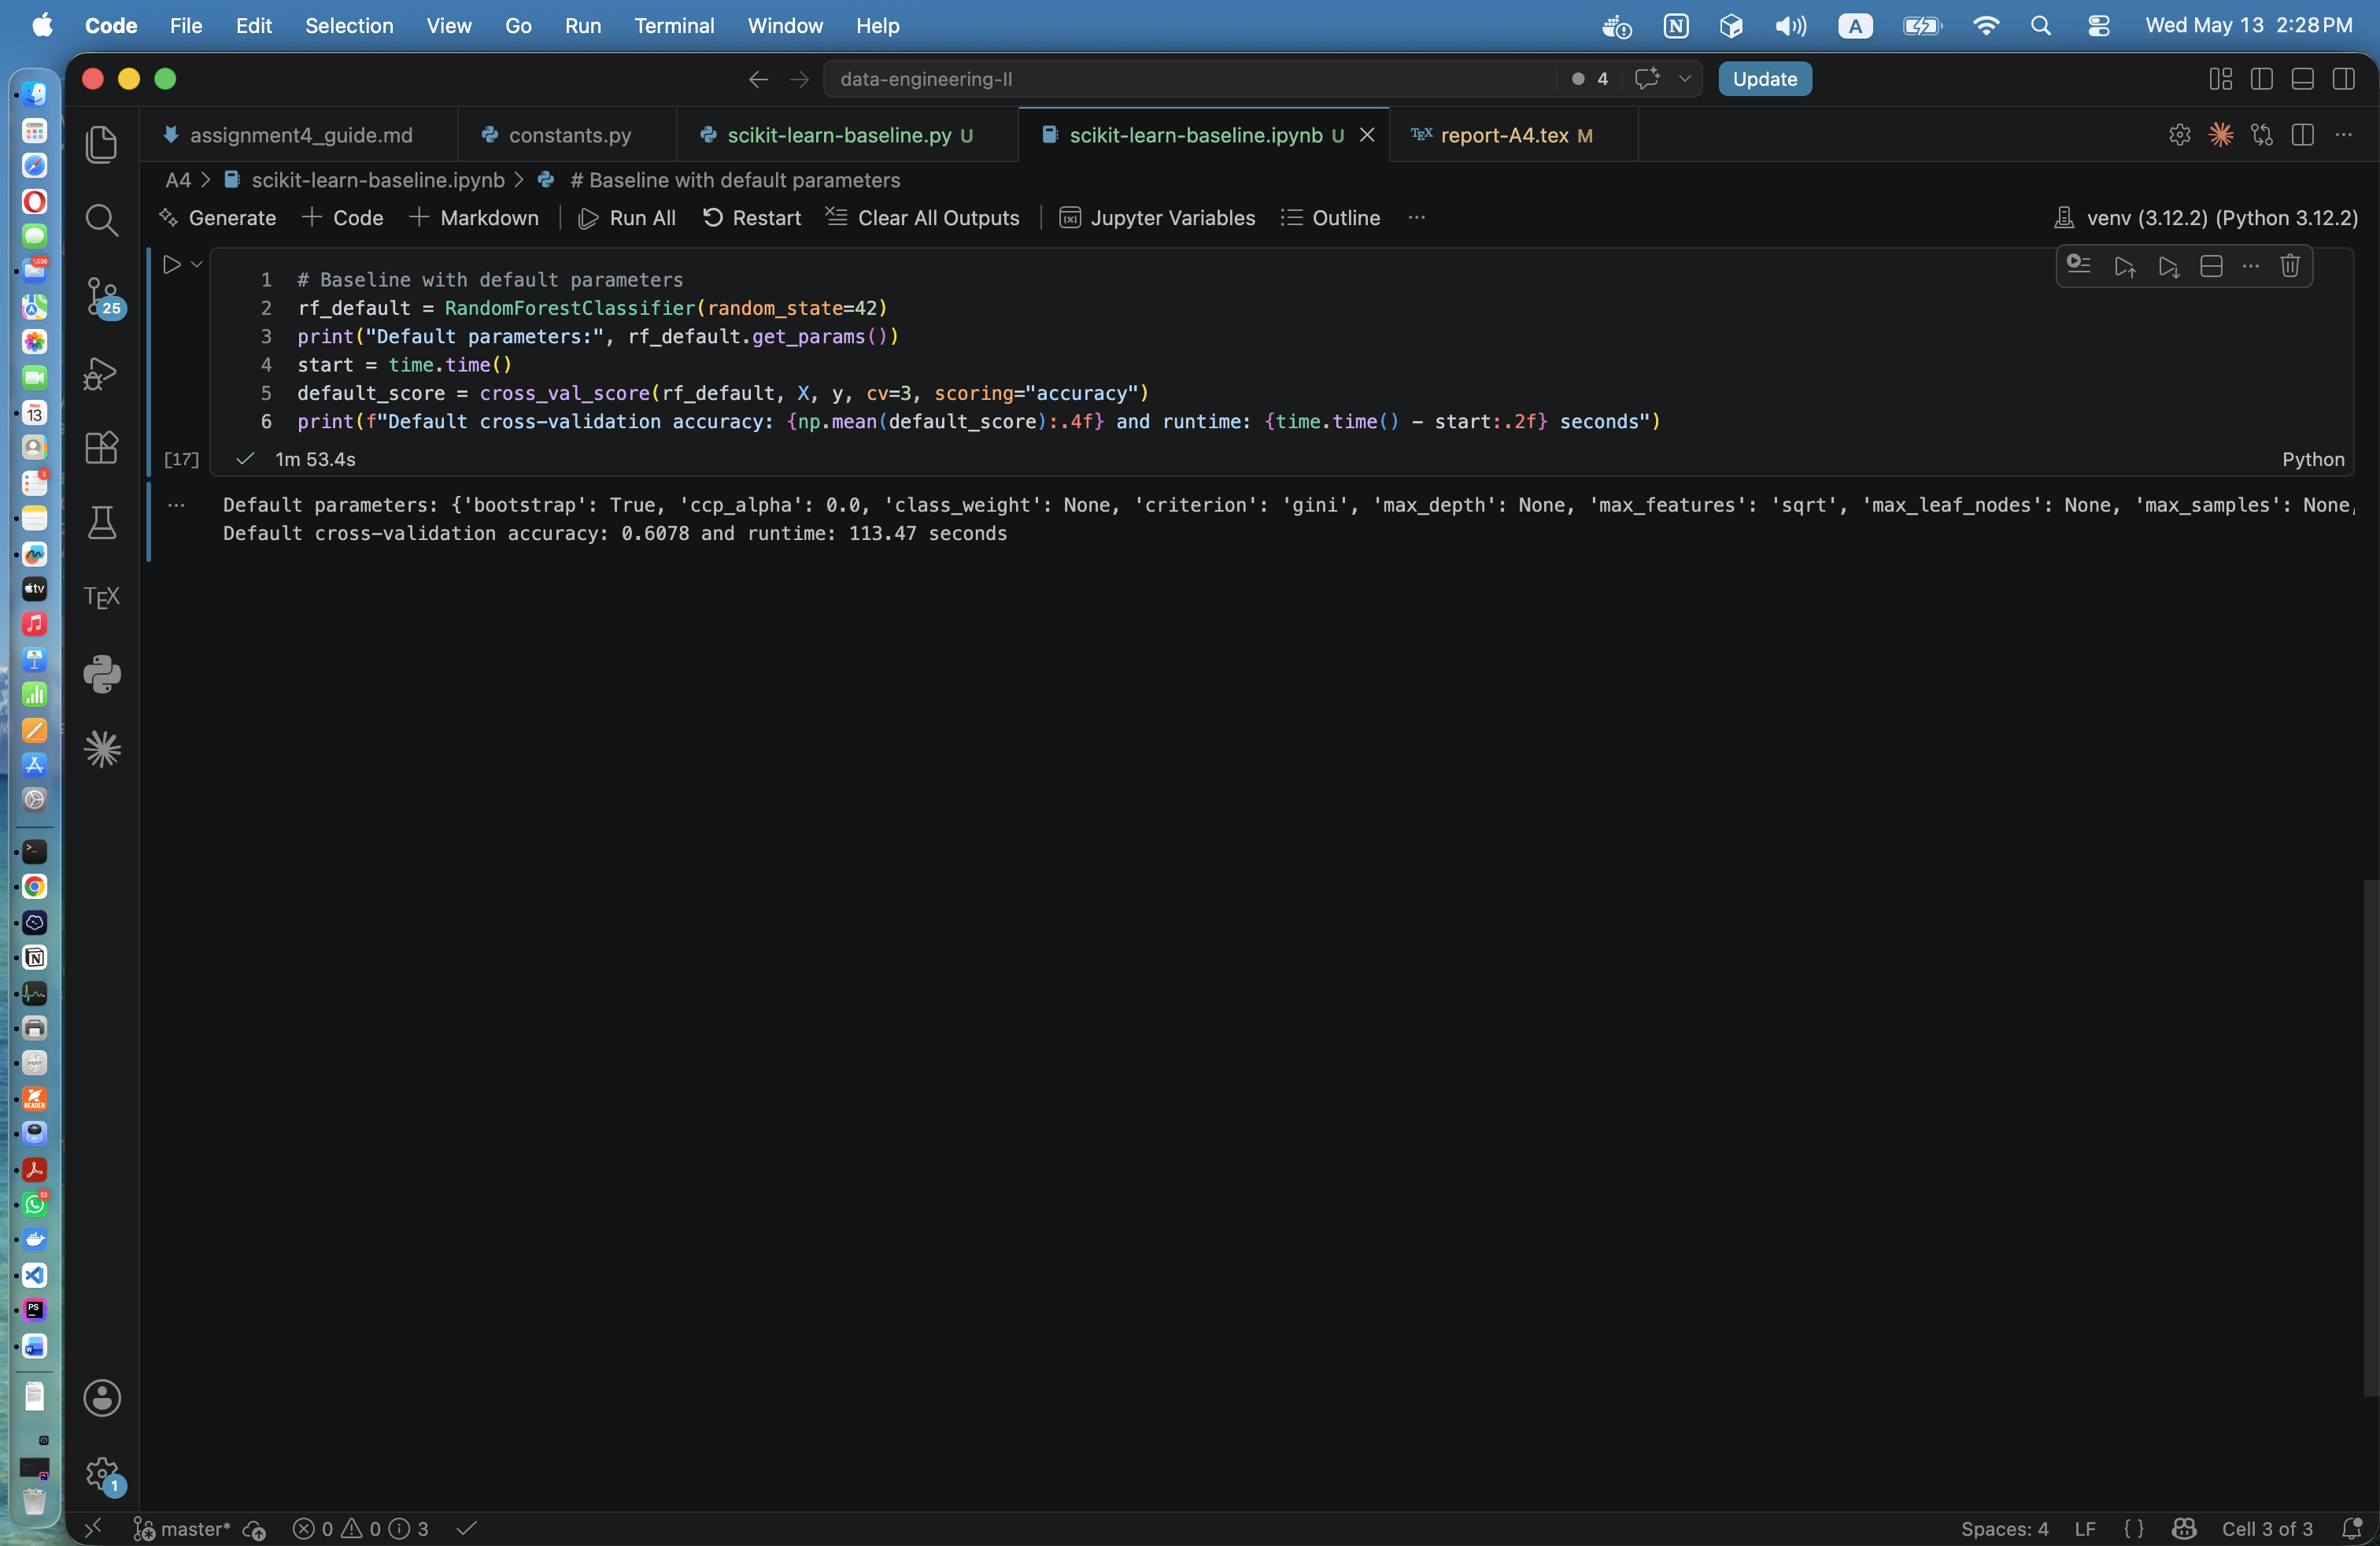
\includegraphics[width=0.95\textwidth]{screenshot-default-model}
  \caption{Training and cross-validation accuracy of the \texttt{RandomForestClassifier}
           using default hyperparameters.}
  \label{fig:default-model}
\end{figure}

\subsubsection{Distributed Hyperparameter Tuning with Ray Tune}

A grid search over the following hyperparameter space was performed using
\textbf{Ray Tune}:

\begin{itemize}[nosep]
  \item \texttt{max\_depth}: \{10, 20, 30\}
  \item \texttt{n\_estimators}: \{50, 100, 150\}
  \item \texttt{ccp\_alpha}: \{0.0, 0.001, 0.01\}
\end{itemize}

This yields $3 \times 3 \times 3 = 27$ candidate combinations, each evaluated with
3-fold cross-validation (81 total fits). The pipeline was deployed on OpenStack VMs of
\emph{small} flavour, with one node acting as the Ray head and the remaining nodes as workers.

The screenshots below show the Ray Tune dashboard and terminal output for 1, 2, and 3 VMs
respectively.

\begin{figure}[H]
  \centering
  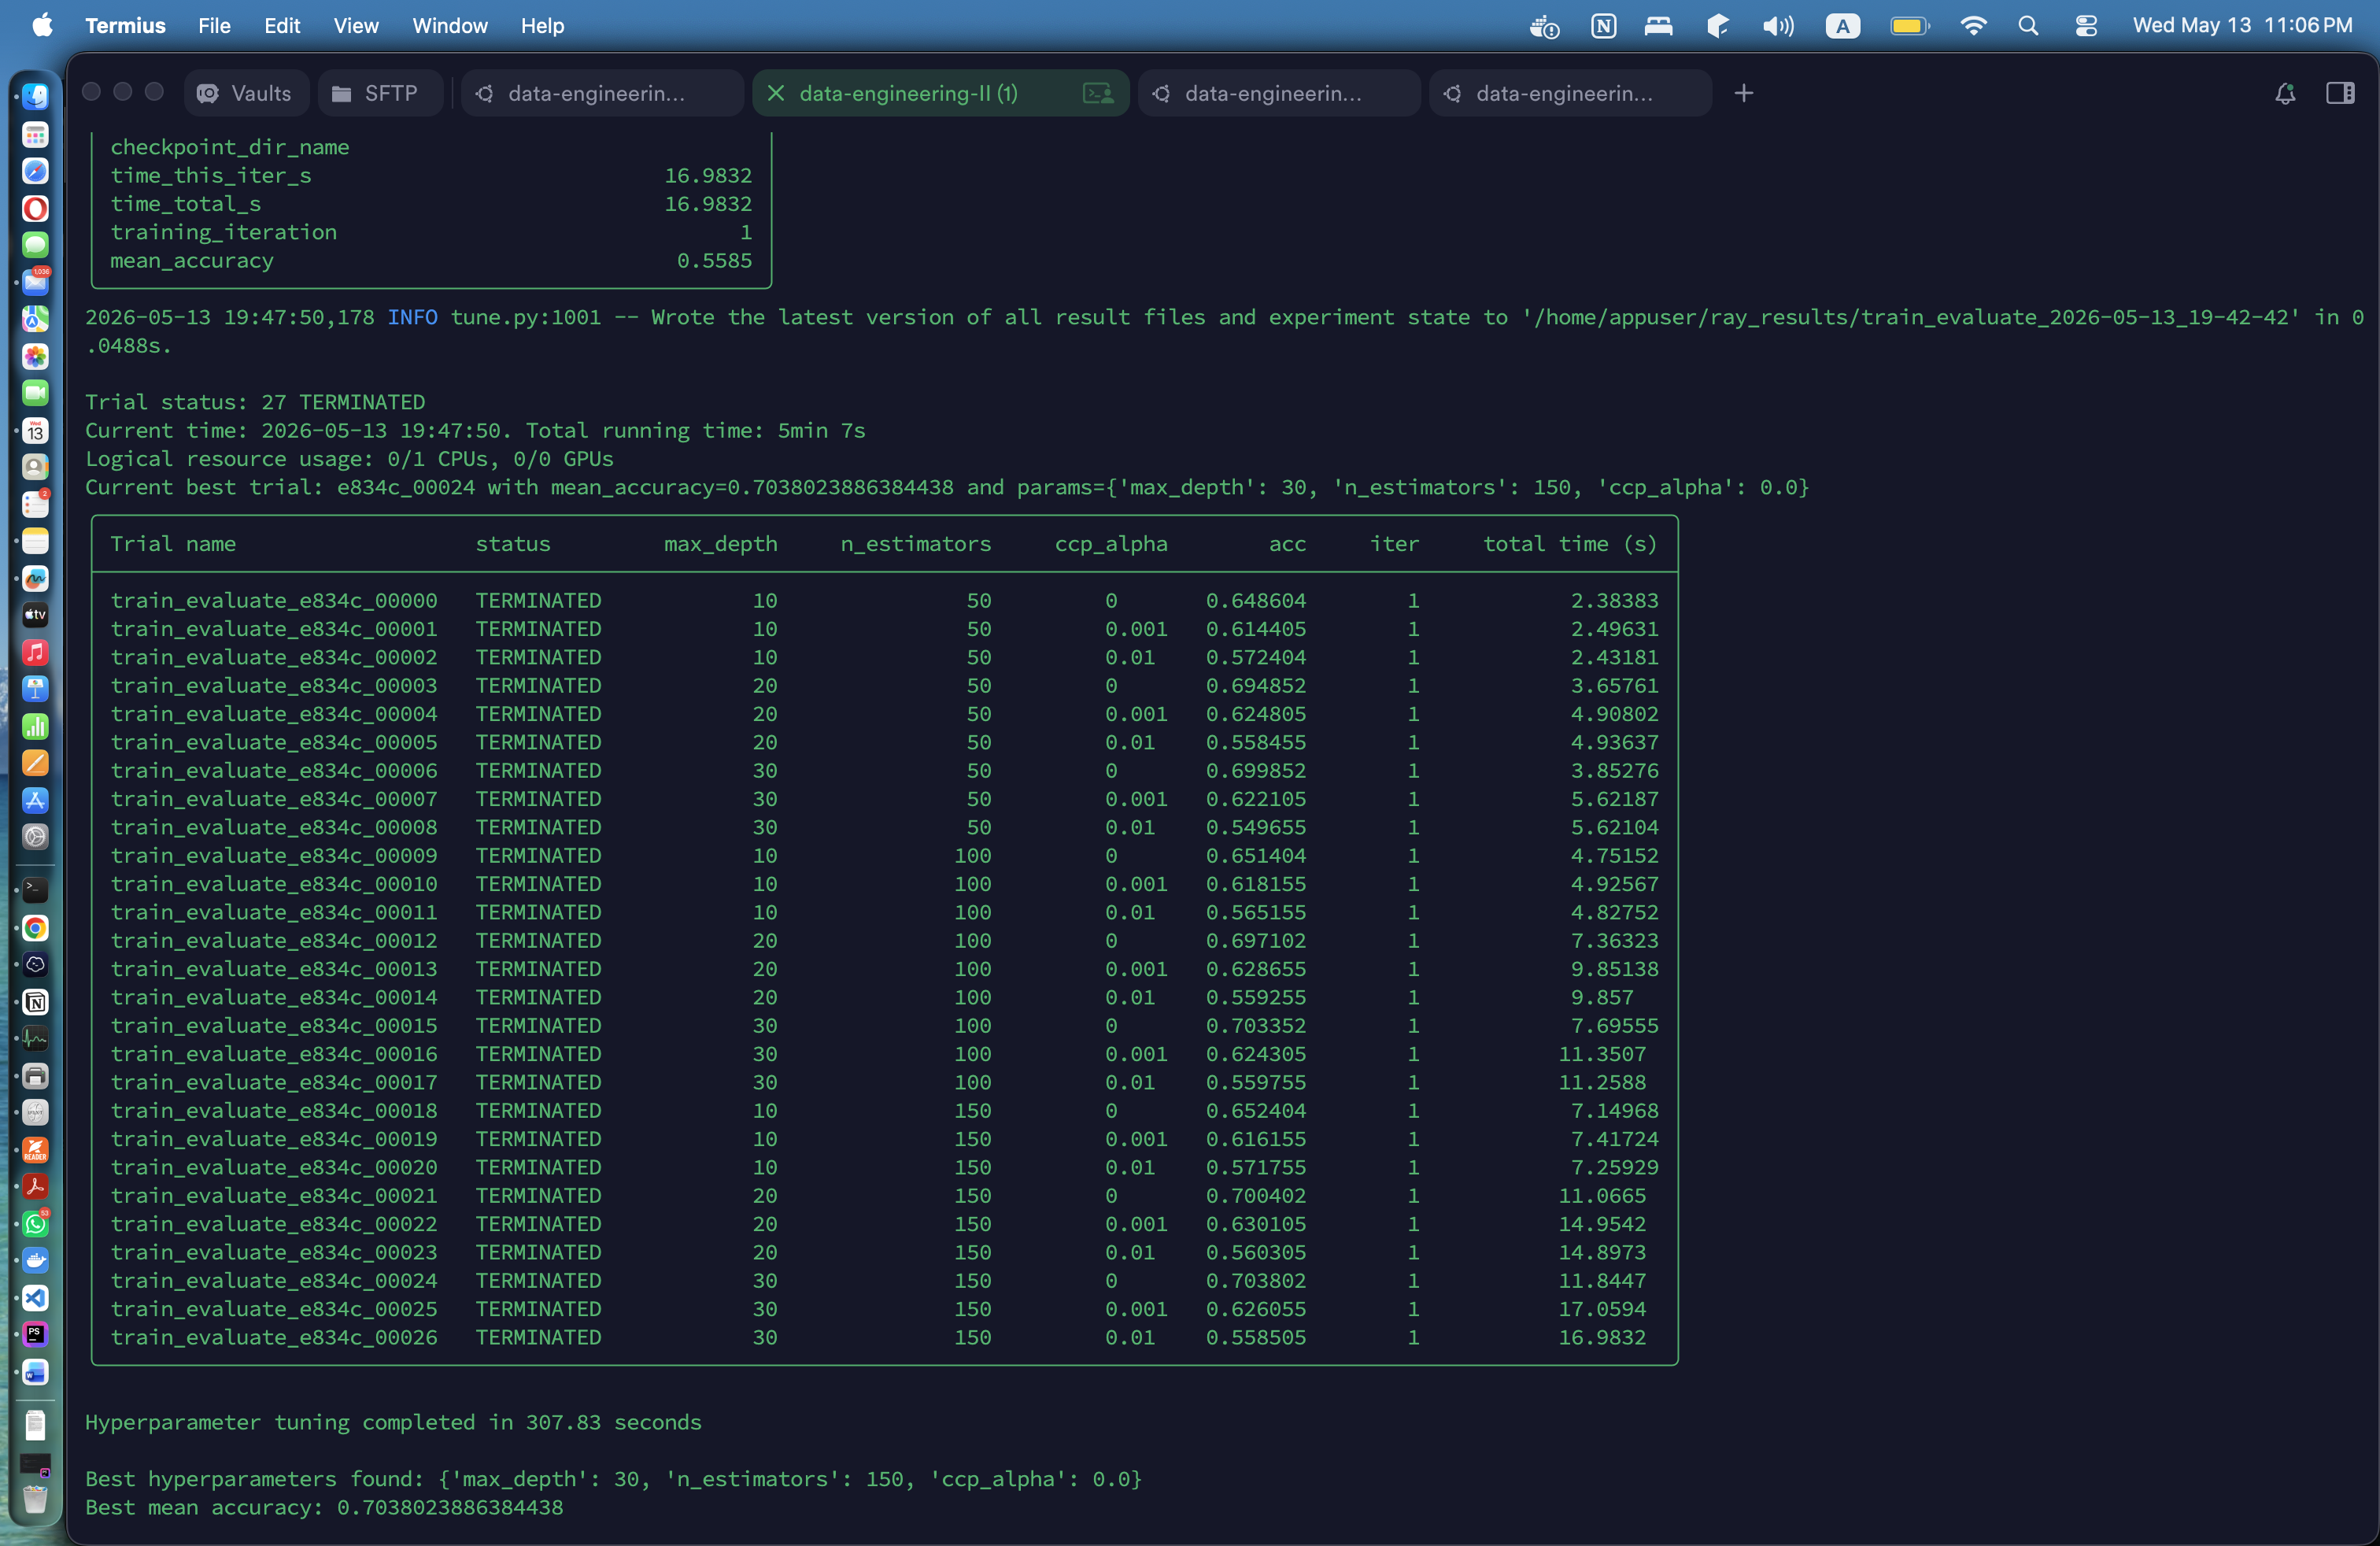
\includegraphics[width=0.95\textwidth]{screenshot-ray-tune-1vm}
  \caption{Ray Tune grid search running on \textbf{1 VM} (head node only).}
  \label{fig:ray-1vm}
\end{figure}

\begin{figure}[H]
  \centering
  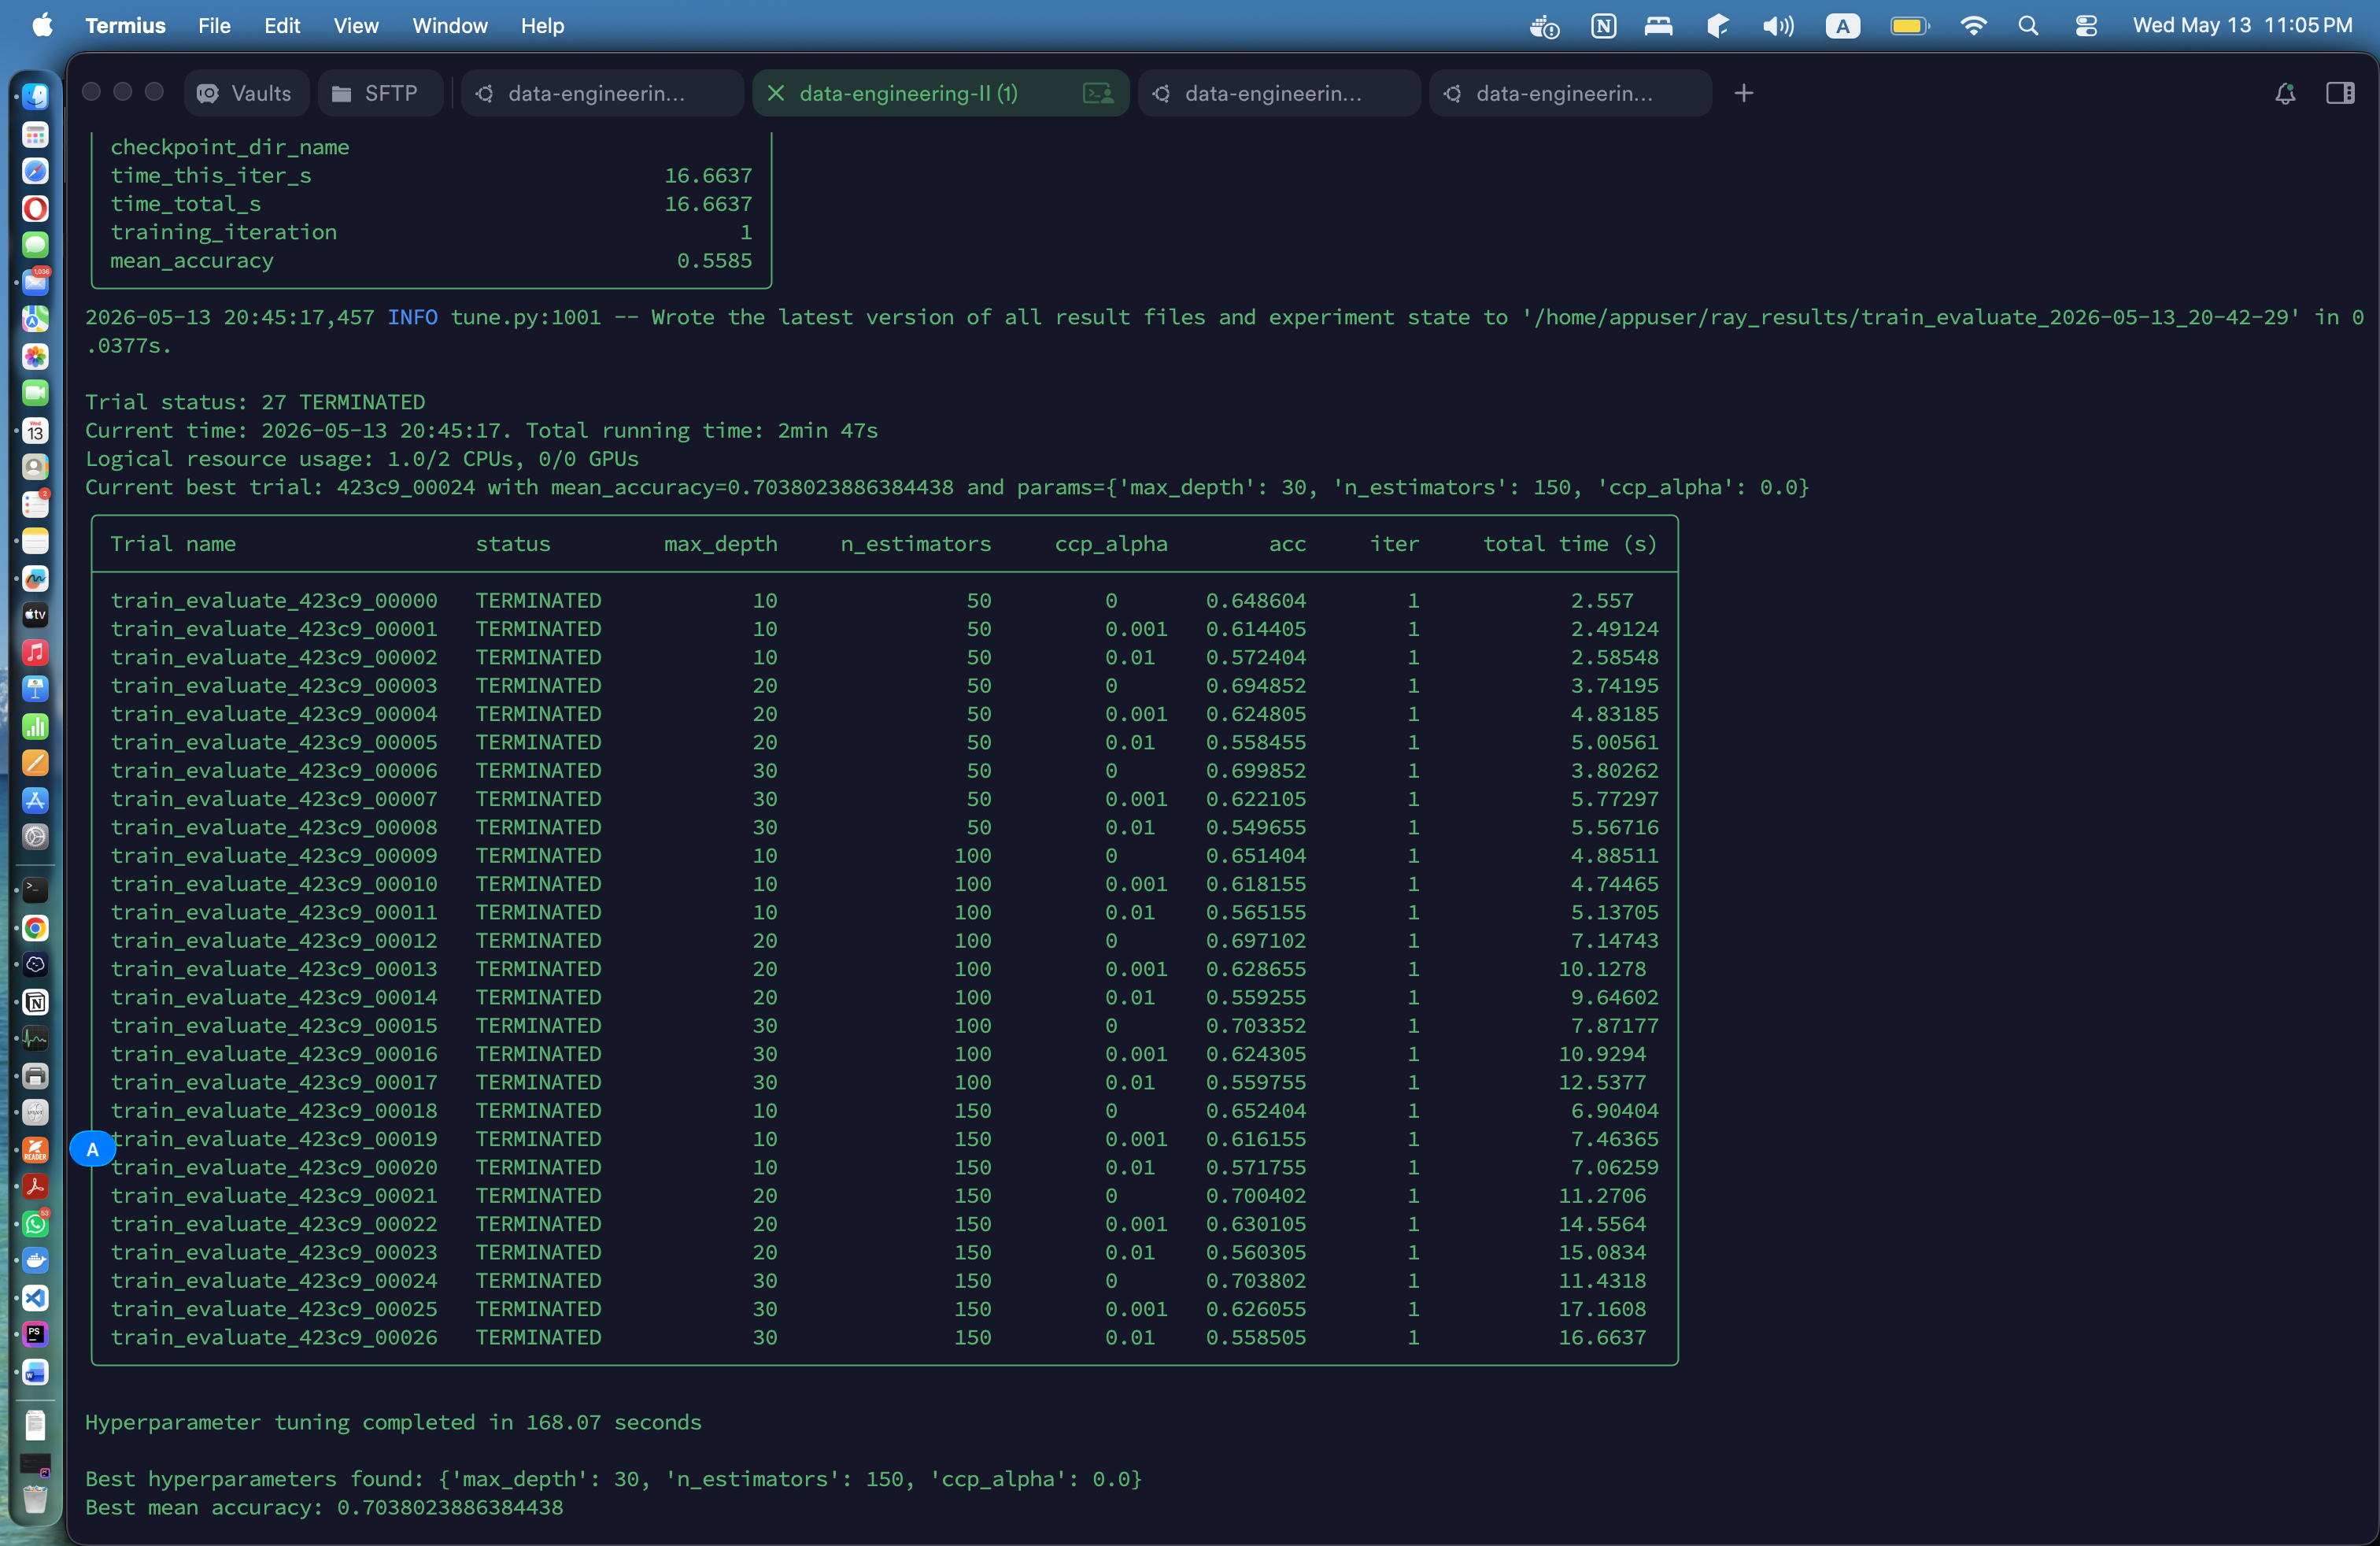
\includegraphics[width=0.95\textwidth]{screenshot-ray-tune-2vm}
  \caption{Ray Tune grid search running on \textbf{2 VMs} (1 head + 1 worker).}
  \label{fig:ray-2vm}
\end{figure}

\begin{figure}[H]
  \centering
  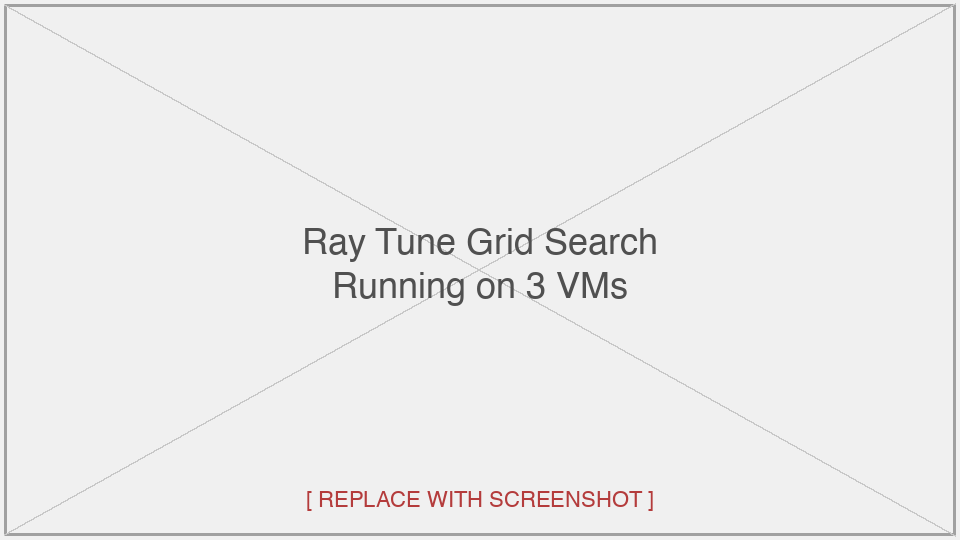
\includegraphics[width=0.95\textwidth]{screenshot-ray-tune-3vm}
  \caption{Ray Tune grid search running on \textbf{3 VMs} (1 head + 2 workers).}
  \label{fig:ray-3vm}
\end{figure}

\subsubsection{Results}

\paragraph{Best hyperparameters and cross-validation score.}

Table~\ref{tab:cv-scores} compares the default configuration against the best
configuration found by the grid search. The tuned model achieved a mean 3-fold
cross-validation accuracy of \textbf{0.7038} -- an improvement of approximately
0.13 percentage points over the default.

\begin{table}[H]
  \centering
  \caption{Cross-validation accuracy: default vs.\ tuned \texttt{RandomForestClassifier}.}
  \label{tab:cv-scores}
  \begin{tabular}{lccc}
    \toprule
    Configuration & \texttt{max\_depth} & \texttt{n\_estimators} & Mean CV Accuracy \\
    \midrule
    Default (\texttt{ccp\_alpha=0.0}) & None  & 100 & 0.7025 \\
    Tuned   (\texttt{ccp\_alpha=0.0}) & 30    & 150 & \textbf{0.7038} \\
    \bottomrule
  \end{tabular}
\end{table}

Table~\ref{tab:top5} lists the top-5 configurations from the grid search.
All top performers use no pruning (\texttt{ccp\_alpha=0.0}), and accuracy
increases monotonically with \texttt{max\_depth}.

\begin{table}[H]
  \centering
  \caption{Top-5 configurations from the Ray Tune grid search.}
  \label{tab:top5}
  \begin{tabular}{ccccc}
    \toprule
    Rank & \texttt{max\_depth} & \texttt{n\_estimators} & \texttt{ccp\_alpha} & Mean CV Accuracy \\
    \midrule
    1 & 30 & 150 & 0.000 & 0.7038 \\
    2 & 30 & 100 & 0.000 & 0.7034 \\
    3 & 20 & 150 & 0.000 & 0.7004 \\
    4 & 30 &  50 & 0.000 & 0.6999 \\
    5 & 20 &  50 & 0.000 & 0.6949 \\
    \bottomrule
  \end{tabular}
\end{table}

\paragraph{Timing comparison across VM counts.}

Table~\ref{tab:timing} shows the wall-clock time and speedup for the full 27-trial
grid search when using 1, 2, and 3 small VMs.

\begin{table}[H]
  \centering
  \caption{Wall-clock time for the full hyperparameter grid search (27 trials, 3-fold CV).}
  \label{tab:timing}
  \begin{tabular}{cccc}
    \toprule
    Number of VMs & CPUs & Wall-clock Time & Speedup vs.\ 1 VM \\
    \midrule
    1 & 1 & 307.83\,s (\textasciitilde{}5\,min 7\,s)  & 1.00$\times$ \\
    2 & 2 & 168.07\,s (\textasciitilde{}2\,min 47\,s) & 1.83$\times$ \\
    3 & 3 & 112.84\,s (\textasciitilde{}1\,min 52\,s) & 2.73$\times$ \\
    \bottomrule
  \end{tabular}
\end{table}

Adding a second VM cut the tuning time by 45\% (1.83$\times$ speedup), and a
third VM achieved a 2.73$\times$ speedup -- near-linear scaling for a 3$\times$
CPU increase. Diminishing returns are visible: the 1$\rightarrow$2 transition
saved 139.76\,s whereas 2$\rightarrow$3 saved only 55.23\,s. This is expected --
the slowest individual trial (\textasciitilde{}17\,s) sets a floor on total time
regardless of the degree of parallelism.

The complete implementation of the distributed hyperparameter tuning pipeline,
including Ray cluster integration and grid search configuration, is shown in
Appendix~\ref{app:tune_random_forest}.

% -----------------------------------------------------------------------------
\subsection{Task 1.2: Distributed Training of Deep Neural Networks}

\subsubsection{TensorFlow Distributed Training Tutorial}

I executed the \textit{Distributed training with TensorFlow} tutorial in Google Colab
using the \texttt{MirroredStrategy} (data parallelism across simulated logical devices).
The screenshot below shows my Colab notebook run confirming successful distributed
training.

\begin{figure}[H]
  \centering
  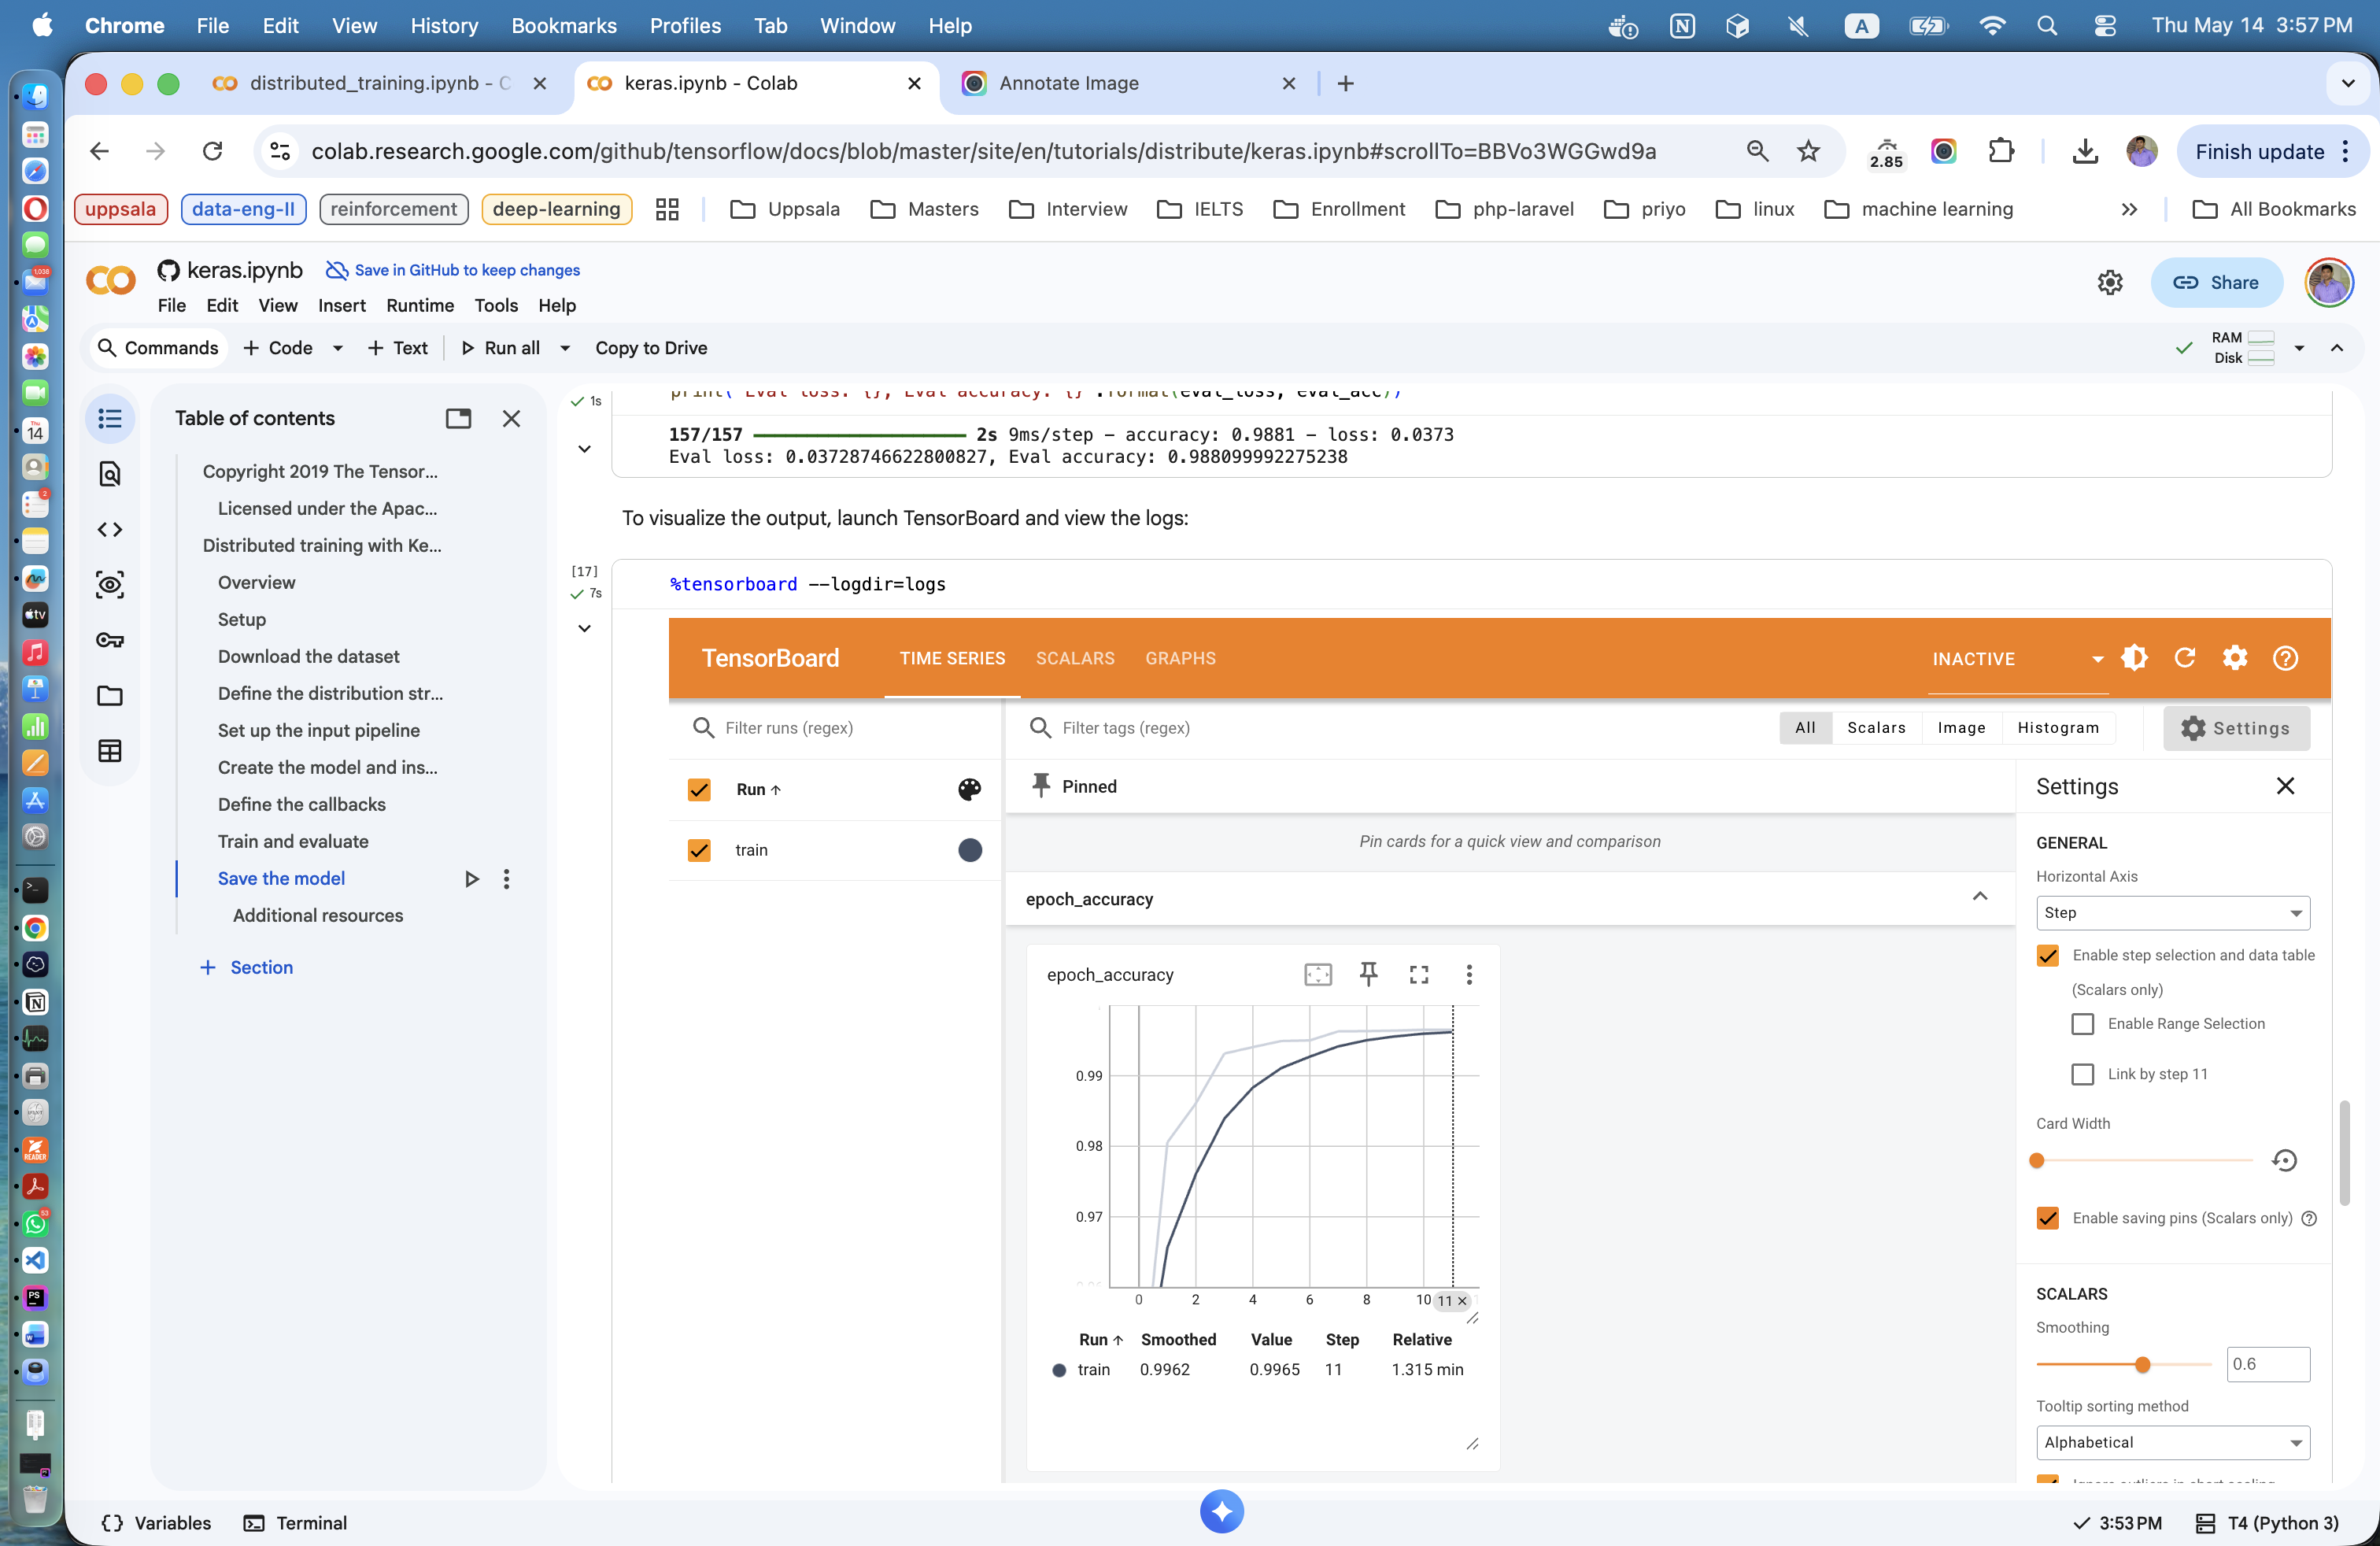
\includegraphics[width=0.95\textwidth]{screenshot-colab-tutorial}
  \caption{Google Colab execution of the TensorFlow distributed training tutorial
           (\texttt{MirroredStrategy}).}
  \label{fig:colab}
\end{figure}

\subsubsection{Data Parallelism vs.\ Model Parallelism}

\textbf{Data parallelism} copies the full model to every device. Each device gets a
different batch of data, computes its own gradients, and then all devices share and
average those gradients before updating the weights. TensorFlow's
\texttt{MirroredStrategy} and PyTorch's \texttt{DistributedDataParallel} both work this
way. This approach works well when the model fits on a single device and the main
bottleneck is the amount of training data. Adding more devices lets training finish
faster.

\textbf{Model parallelism} splits the model itself across devices. Different layers or
parts of the model live on different devices. This is needed when the model is too large
to fit on one device, such as very large language models with billions of parameters.
Two common ways to do this are pipeline parallelism (each device handles a group of
layers in sequence) and tensor parallelism (weight matrices are split across devices).

\textbf{When to distribute a single training run vs.\ the whole tuning sweep:}
If training one model configuration already takes too long on a single device, it makes
sense to spread that one run across multiple devices using data or model parallelism.
On the other hand, if each training run is fast, it is better to run many configurations
in parallel -- one per worker -- instead of adding communication overhead to every forward
pass. In my experiments with Ray Tune and the random forest, individual runs were fast
enough that I parallelised across configurations rather than within a single run.

% =============================================================================
\section{Task 2: Federated Learning }
% =============================================================================

\subsection{Simulation Setup}

I launched two \textit{Datasite} nodes locally using \textbf{PySyft $\geq$ 0.8}
(\texttt{dev\_mode=True} to bypass manual approval) representing \emph{Client~A} and
\emph{Client~B}. I partitioned the MNIST training set (60\,000 images) into two
non-overlapping halves: samples 0--29\,999 for Client~A and samples 30\,000--59\,999
for Client~B.

I uploaded each partition to its respective datasite using the dataset upload API.
PySyft~0.8 persists large tensors in blob storage on the server before registering
them. I received back only an asset pointer -- a UUID reference to the data stored
on the server -- never the raw tensor bytes.

\begin{figure}[H]
  \centering
  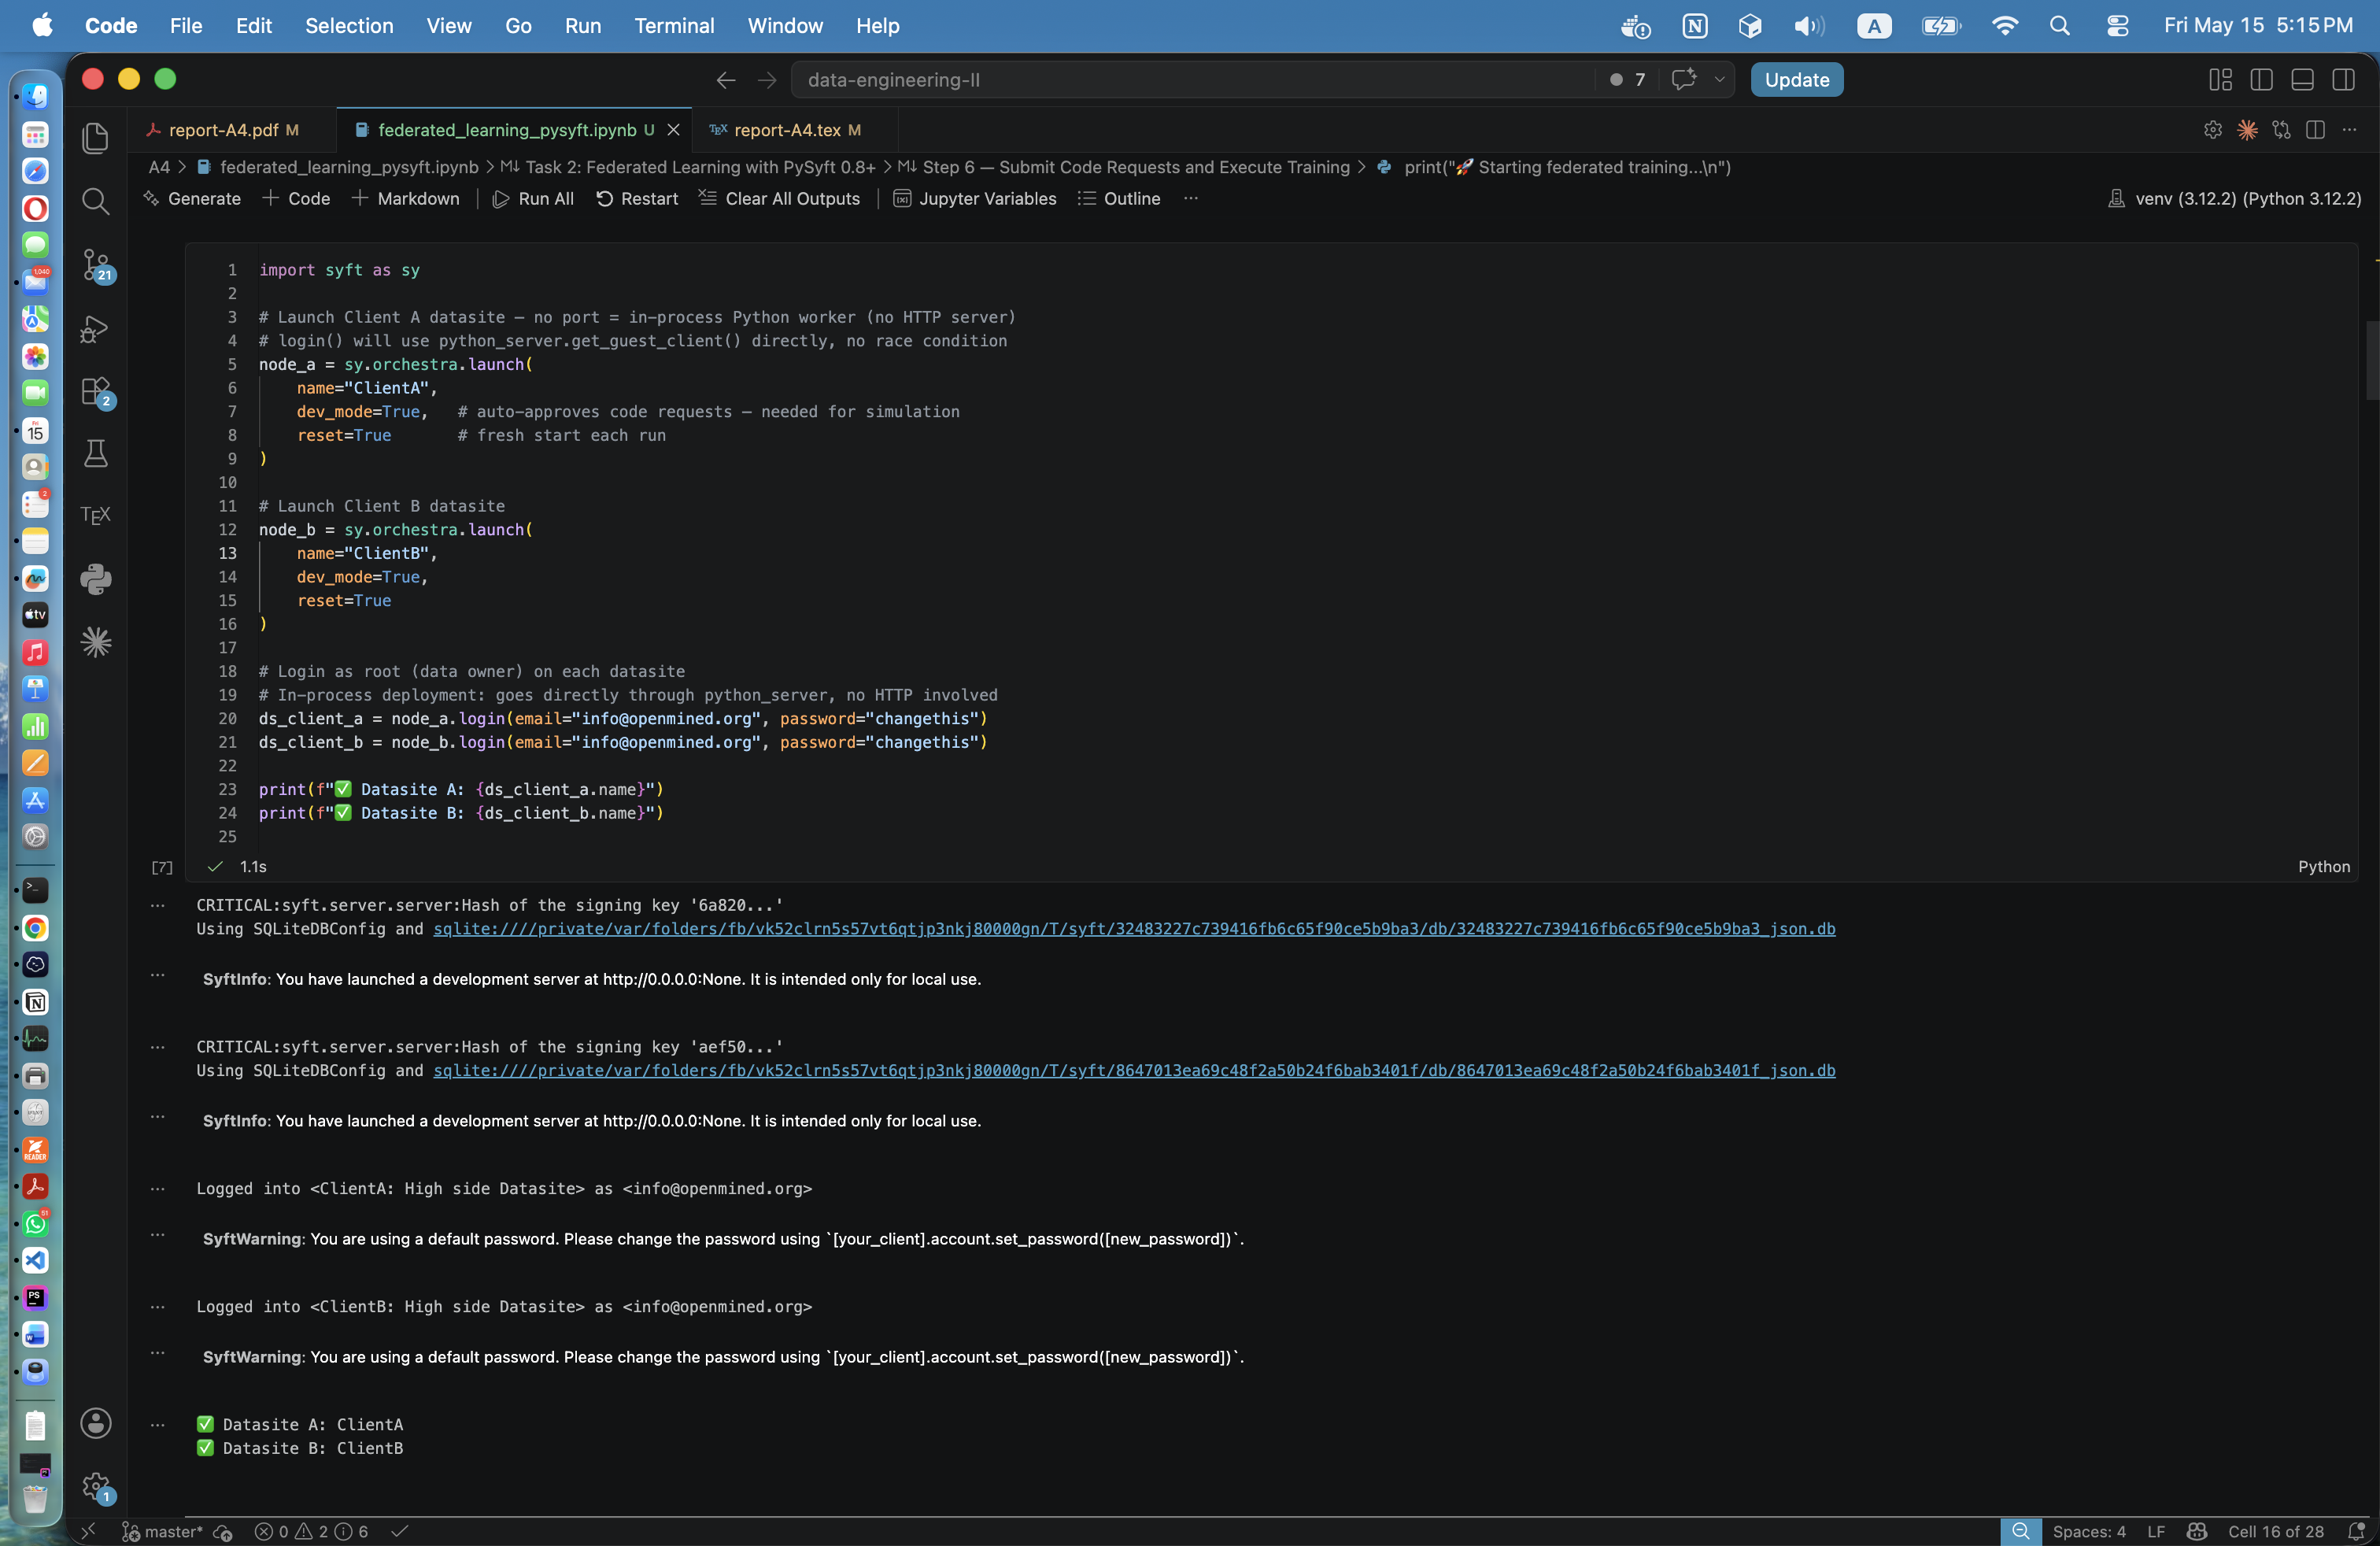
\includegraphics[width=0.95\textwidth]{screenshot-pysyft-setup}
  \caption{PySyft Datasite workers (Client~A and Client~B) initialised with
           non-overlapping MNIST partitions.}
  \label{fig:pysyft-setup}
\end{figure}

\subsection{Federated Training}

I defined a \texttt{SimpleCNN} convolutional network (one convolutional block with
16 filters, one max-pool layer, and two fully-connected layers culminating in 10-class
logits). I registered each worker's training function using the \texttt{@syft\_function} decorator.
The \texttt{ExactMatch} input policy locks the function to the pre-approved \texttt{Asset}
pointers only. The \texttt{SingleExecutionExactOutput} output policy restricts the return
value to the declared \texttt{state\_dict} only. Both clients trained for \textbf{3 epochs}
with SGD (lr$\,=\,0.01$, momentum$\,=\,0.9$) and batch size 256. Each function returned a
plain \texttt{dict} of detached tensors, as required by PySyft's serialiser.

I then collected the two returned state dicts and performed a single round of
\textbf{FedAvg} -- parameter-wise weighted average with equal weights (0.5 / 0.5, since
both workers held 30\,000 samples):
\[
  \theta_{\text{global}} = \tfrac{1}{2}\,\theta_A + \tfrac{1}{2}\,\theta_B
\]
The aggregated weights were loaded into a fresh \texttt{SimpleCNN} instance to form the
global model. Total wall-clock time for both remote training calls was \textbf{13.5\,s}.

\begin{figure}[H]
  \centering
  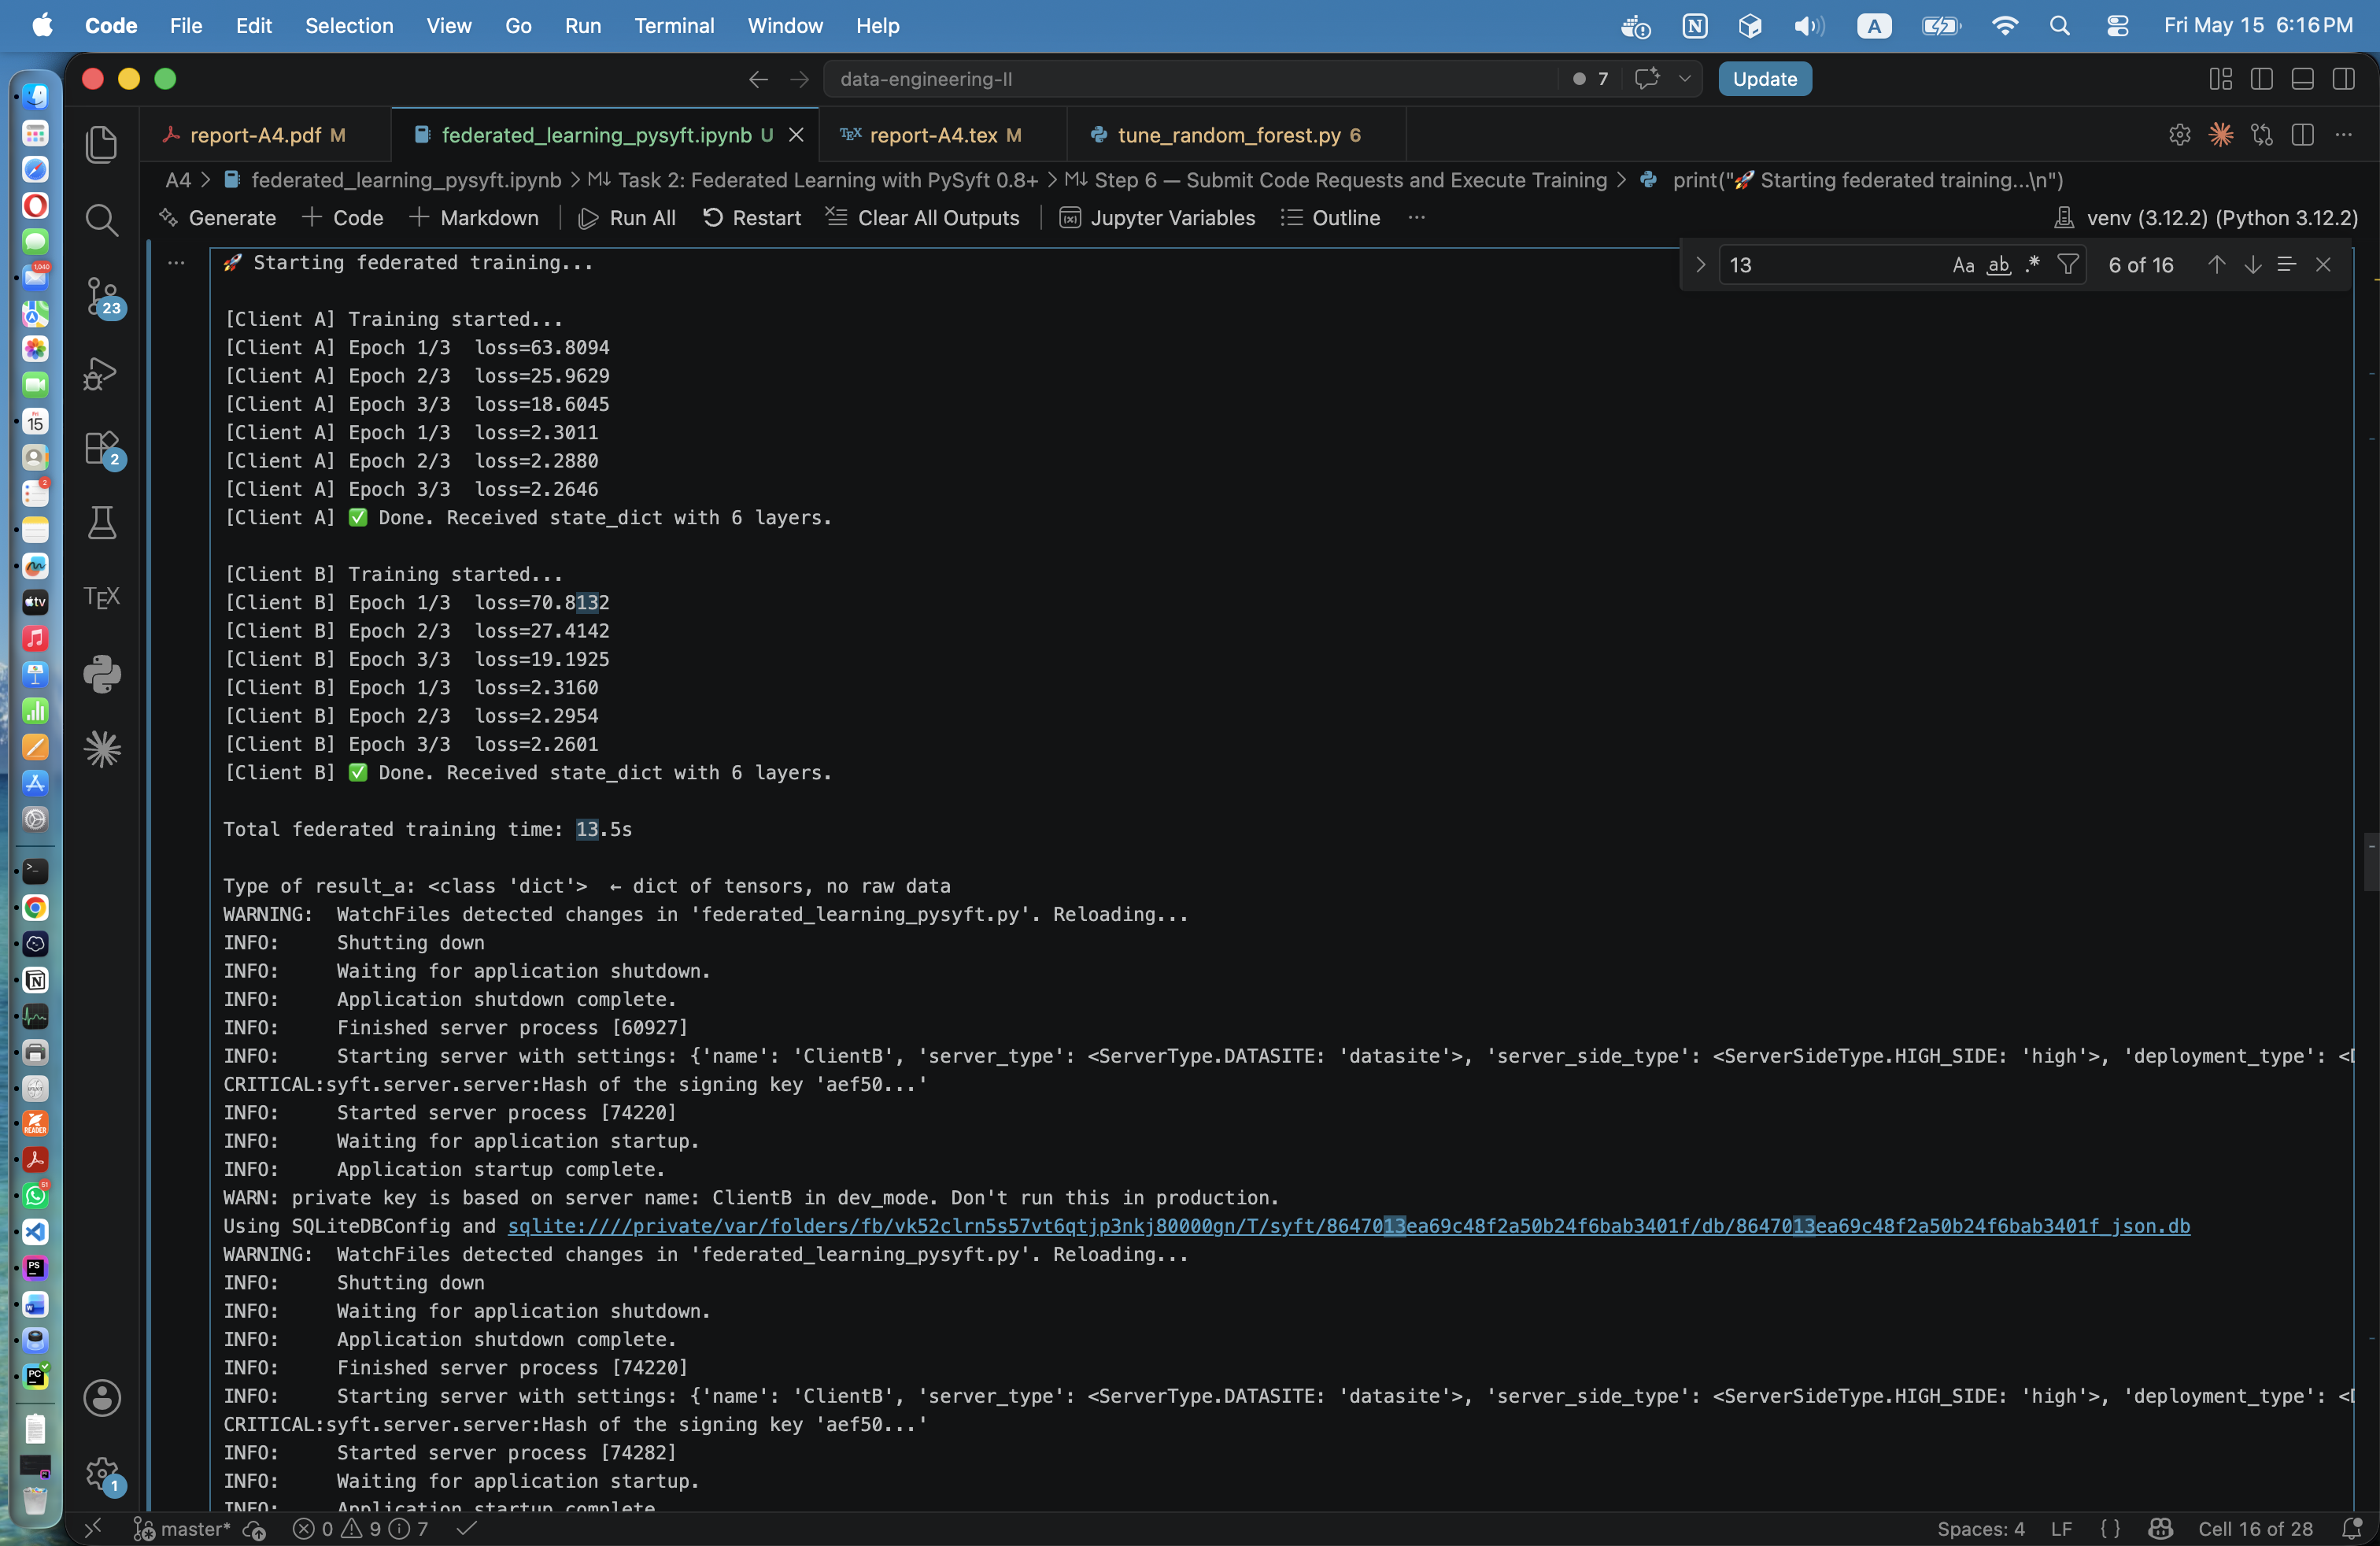
\includegraphics[width=0.95\textwidth]{screenshot-federated-training}
  \caption{Terminal output showing per-worker local loss over 3 epochs and the
           FedAvg aggregation step.}
  \label{fig:fl-training}
\end{figure}

\subsection{Analysis}

\subsubsection{How PySyft's \texttt{ActionObject} Prevents Raw Data Access}

In PySyft~0.8+, I never held the raw tensor data directly. When I called
\texttt{upload\_dataset()}, the raw tensors were stored in blob storage on the
Datasite server via \texttt{TwinObject.\_save\_to\_blob\_storage()}. I received
back only an \texttt{Asset} -- a UUID pointer (\texttt{action\_id}) -- with no
access to the underlying pixel values.

Any code that accesses private data must be submitted as a \texttt{@syft\_function}
decorated function. Two policies enforce the privacy boundary:
\begin{itemize}[nosep]
  \item \textbf{\texttt{input\_policy = ExactMatch(...)}}: the function can only be
        called with the pre-approved \texttt{Asset} pointers; arbitrary tensor
        injection is blocked.
  \item \textbf{\texttt{output\_policy = SingleExecutionExactOutput()}}: only the
        declared return value (\texttt{state\_dict}) is allowed out of the node;
        no intermediate tensors or raw data can be returned.
\end{itemize}

In production, the Datasite administrator must manually approve each code request
via the PySyft web UI before execution. I used \texttt{dev\_mode=True} to
auto-approve requests for simulation purposes, but the privacy enforcement is
identical in both modes. The net effect is that the data owner retains full
governance: I submitted an auditable function, and only approved, policy-conforming
results left each node.

\subsubsection{Federated Model Accuracy vs.\ Single-Worker Baseline}

All three models were evaluated on the held-out MNIST test set (10\,000 samples).
Table~\ref{tab:fl-accuracy} summarises the results.

\begin{table}[H]
  \centering
  \caption{Test accuracy on MNIST for federated and local-only models.}
  \label{tab:fl-accuracy}
  \begin{tabular}{lcc}
    \toprule
    Model & Training data & Test accuracy \\
    \midrule
    Federated (FedAvg, single round) & 60\,000 (split) & 80.52\% \\
    Local-only (Client~A)            & 30\,000         & \textbf{96.15}\% \\
    Local-only (Client~B)            & 30\,000         & 96.06\% \\
    \bottomrule
  \end{tabular}
\end{table}

\begin{figure}[H]
  \centering
  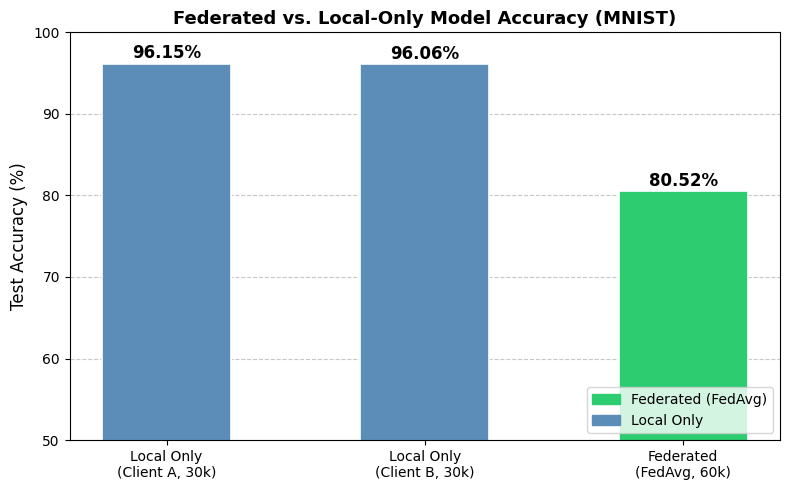
\includegraphics[width=0.85\textwidth]{screenshot-accuracy-comparison}
  \caption{MNIST test accuracy: Federated model (FedAvg) achieved 80.52\%, compared to local-only baselines (Client~A: 96.15\%, Client~B: 96.06\%).}
  \label{fig:accuracy}
\end{figure}

\textbf{The federated model underperformed both local baselines by approximately
15.6 percentage points} (80.52\% vs.\ 96.15\% for Client~A and 96.06\% for Client~B).
This result is counterintuitive at first but has a well-known explanation: FedAvg
averages model weights in parameter space. When two networks are trained
\emph{independently from different random initialisations}, their weight spaces do not
align -- different neurons learn the same feature in different positions, and averaging
their weights yields a model that represents no feature well. This phenomenon is known
as \emph{weight-space incompatibility} or \emph{permutation misalignment}.

In canonical FL, the global model is \emph{broadcast} to all workers at the start of
each round. All workers then start from the same weights, and local training moves each
model only a small number of steps away. Averaging these nearby points in weight space
produces a coherent result. My simulation skips this broadcast step: each worker trains
from scratch with a different random initialisation. Their weight spaces therefore
divide completely, and FedAvg over two such independent models is expected to perform
poorly.

Despite this, my experiment correctly demonstrates the privacy guarantee: neither
worker ever shared raw pixels with the other or with the coordinator.

\subsection{Written Reflection}

\subsubsection{Federated Learning vs.\ Distributed ML: Statistical and System
               Heterogeneity}

Regular distributed ML (for example, data-parallel SGD with a parameter server or a Ray
cluster) assumes two things: the data is spread evenly across all workers, and all
workers have similar hardware and network speed. Federated Learning breaks both of these
assumptions.

\textbf{Statistical heterogeneity} (\emph{non-IID data}): Each FL participant has
different data. For example, a hospital in one city sees different patients than one in
another city. Because the data is not evenly distributed, each worker's local model
updates point in different directions. When these updates are averaged, the global model
can be biased toward the workers with more data. This problem does not happen in
data-centre distributed ML, where data is shuffled evenly before training starts.
Algorithms such as FedProx and SCAFFOLD are designed to reduce this bias.

\textbf{System heterogeneity} (\emph{stragglers and availability}): FL clients have
very different hardware. One client might be a slow smartphone and another might be a
powerful server. In synchronous training, the system must wait for the slowest worker
(\emph{straggler problem}). In asynchronous training, some workers may send outdated
updates. Data-centre distributed ML avoids this because all machines are controlled and
similar.

\textbf{Relation to the Parameter Server strategy}: In the Parameter Server (PS)
approach, a central server holds the global model. Workers download the model, compute
updates on their local data, and send the updates back. FL looks similar to this -- the
aggregation server acts like a PS -- but there are three key differences:
\begin{enumerate}[nosep]
  \item \textbf{Privacy}: In PS, raw gradients go to the server. These gradients can be
        used to reconstruct private training data (gradient inversion attacks). In FL,
        only model weights (state dicts) are shared -- the server never sees the raw
        data. PySyft enforces this with \texttt{ActionObject} and \texttt{output\_policy}.
  \item \textbf{Data distribution}: PS assumes data is spread evenly across trusted
        machines. FL must handle uneven data across independent organisations.
  \item \textbf{Trust model}: PS workers are trusted machines inside one organisation.
        FL participants are separate entities with their own data rules. This is why FL
        systems need code approval workflows, differential privacy, and secure
        aggregation in real deployments.
\end{enumerate}

% =============================================================================
\begin{appendices}

\section{Code Files}

\subsection{random\_forest\_baseline.py}

This script implements the baseline scikit-learn model, evaluating the
\texttt{RandomForestClassifier} with default hyperparameters using 3-fold
cross-validation on the cover-type dataset.

\lstinputlisting[style=python, caption=random\_forest\_baseline.py]{../random_forest_baseline.py}

\subsection{tune\_random\_forest.py}
\label{app:tune_random_forest}

This script implements distributed hyperparameter tuning with Ray Tune.
It loads the dataset, places it in Ray's object store, and launches a
$3 \times 3 \times 3$ grid search over \texttt{max\_depth},
\texttt{n\_estimators}, and \texttt{ccp\_alpha}, distributing trials
across all nodes in the Ray cluster.

\lstinputlisting[style=python, caption=tune\_random\_forest.py]{../tune_random_forest.py}

\subsection{OpenStack Client Configuration}

\subsubsection{constants.py}

Configuration constants for OpenStack instance provisioning:

\lstinputlisting[style=python, caption=constants.py]{../openstack-client/constants.py}

\subsubsection{start\_instance.py}

OpenStack Nova client script for provisioning Ray cluster instances:

\lstinputlisting[style=python, caption=start\_instance.py]{../openstack-client/start_instance.py}

\subsection{federated\_learning\_pysyft.py}

This script is the Python conversion of the \texttt{federated\_learning\_pysyft.ipynb}
Jupyter notebook. It contains the complete federated learning simulation: launching two
PySyft Datasites, partitioning and uploading MNIST data, defining and submitting
\texttt{@syft\_function} training jobs, performing FedAvg aggregation, and evaluating
the federated and local-only models.

\lstinputlisting[style=python, caption=federated\_learning\_pysyft.py]{../federated_learning_pysyft.py}

\subsection{Ansible Playbooks}

\subsubsection{install\_ray.yml}

Ansible playbook to install Ray and dependencies on cluster nodes:

\lstinputlisting[style=yaml, caption=install\_ray.yml]{../openstack-client/ansible/install_ray.yml}

\end{appendices}

% =============================================================================
\end{document}

